\documentclass{article}
\usepackage{polski}
\usepackage{blindtext}
\usepackage{amsmath}
\usepackage{mathtools}
\usepackage{graphicx} 
\usepackage{wrapfig}
\usepackage{amssymb}
\usepackage{multirow}
\usepackage[usenames,dvipsnames,svgnames,table]{xcolor}
\usepackage{float}
\usepackage[caption = false]{subfig}
\usepackage{caption}
\newcommand\tab[1][1cm]{\hspace*{#1}}
\usepackage[a4paper, left=2.5cm, right=2.5cm, top=2.5cm, bottom=2.5cm, headsep=1.2cm]{geometry}

\usepackage{titling}
\newcommand{\subtitle}[1]{%
  \posttitle{%
    \par\end{center}
    \begin{center}\large#1\end{center}
    \vskip0.5em}%
}


\begin{document}
\title{\textsc{Sprawozdanie - laboratorium 6}}
\subtitle{\textbf{Wyznaczanie zer wielomianu metodą siecznych}}
\author{Zuzanna Grzesik}
\date{8 kwietnia 2020}

\maketitle	

\section{Wstęp teoretyczny}	
\subsection{Metoda Regula Falsi}
Jest to metoda, która umożliwia znalezienie pierwiastków funkcji nieliniowej. Nazwa  ta oznacza "fałszywą linię prostą/regułę", ponieważ metoda ta wykorzstuje fałszywe założenie o lokalnej liniowości funkcji. Dodatkowo należy również założyć, że:
\begin{itemize}
\item w przedziale $[a, b]$ funkcja ma tylko jeden pierwiastek pojedynczy,
\item $f(a) \cdot f(b) < 0$,
\item funkcja jest klasy $C^2$,
\item pierwsza i druga pochodna nie zmieniają znaku w przedziale $[a, b]$. 
\end{itemize}

Algorytm przebiega następująco:

\begin{enumerate}
\item Przez punkty $A = (a, f(a))$ i $B = (b, f(b))$ przeprowadzamy cięciwę.
\item Punkt przecięcia cięciwy z osią OX $x_0$ przyjmowany jest jako pierwsze przybliżenie pierwiastka i można opisać jego wartość wzorem:
\begin{equation}
x_0 = a - \frac{f(a)}{f(b) - f(a)} (b - a)
\end{equation}
\item Jeżeli przybliżenie jest wystarczająco dobre, czyli $f(x_0) = 0$ lub $\epsilon_{k+1} = | x_{k+1} - x_{k} |$ jest bardzo małe (np. mniejsze niż $10^{-6}$), czyli różnica pomiędzy kolejnymi przybliżeniami jest już znikoma - algorytm kończy się.
\item Jeżeli nie jest odpowiednio dobre, to prowadzona jest nowa cięciwa przez punkty $(x_0, f(x_0))$ oraz punkt A lub B, w zależności od tego, który z nich ma drugą współrzędną o znaku przeciwnym do $f(x_0)$.
\item Wyznaczane jest przecięcie nowej cięciwy z osią OX $(x_k)$ i wracamy do punktu 3.
\end{enumerate}


Kolejne przybliżenia pierwiastka $x$ można więc opisać wzorem:
\begin{equation}
\begin{cases} 
	x_{k+1} = x_k - \frac{f(x_k)}{f(b) - f(x_k)} (b - x_k) & \text{gdy} f(b)f(x_k) \geq 0  \\
	x_{k+1} = x_k - \frac{f(x_k)}{f(a) - f(x_k)} (a - x_k) & \text{gdy} f(a)f(x_k) \geq 0
\end{cases}
\end{equation}
gdzie $x_0 = a$.

\subsection{Metoda siecznych}
Metoda ta jest modyfikacją metody Regula Falsi, opisanej w punkcie (1.1). Różnica pomiędzy nimi polega na tym, że sieczną przeprowadza się przez dwa ostatnie przybliżenia $x_k$ oraz $x_{k+1}$. Kolejne przybliżenia wyznacza się za pomocą wzoru:
\begin{equation}
x_{k+1} = x_k - \frac{f(x_k)(x_k - x_{k-1})}{f(x_k) - f(x_{k-1})}. 
\end{equation}
Zbieżność tej metody jest większa niż metody Regula Falsi. 
\par Metodę siecznych można zmodyfikować by móc szukać również pierwiastków wielokrotnych. Jeżeli nie znamy krotności pierwiastka, musimy w tym celu zbadać zera funkcji $u(x) = f(x)/f'(x)$. We wzorze na kolejne przybliżenia pierwiastku należy dokonać zamiany funkcji $f(x)$ na $u(x)$. W efekcie wzór wygląda następująco:
\begin{equation}
x_{k+1} = x_{k} - \frac{x_k - x_{k-1}}{u(x_k) - u(x_{k-1})} u(x_k).
\end{equation}


\section{Zadanie do wykonania}
\subsection{Opis problemu}
Zadaniem w trakcie laboratoriów było wyznaczenie wszystkich pierwiastków równania nieliniowego postaci:
\begin{equation}
	f(x) = (x - 1.2)(x - 2.3)(x - 3.3)^2 ,
\end{equation}
korzystając z metody siecznych. 
\par Na początek należało stworzyć wykres funkcji $f(x)$, dla $x \in [0.9, 3.7]$. Następnie należało napisać program do wyznaczania pierwiastków wielomianu (dla podwójnej precyzji). Wyznaczanie zer miało odbywać się dwoma metodami:
\begin{enumerate}
\begin{enumerate}
\item niemodyfikowaną metodą siecznych
\item modyfikowaną metodą siecznych.
\end{enumerate}
\end{enumerate}
Dla niemodyfikowanej metody siecznych korzystaliśmy ze wzoru (3) dla obliczania kolejnych przybliżeń pierwiastka.
Natomiast dla modyfikowanej metody siecznych funkcje $f(x)$ należało zastąpić funkcją $u(x)$ i skorzystać ze wzoru (4)
gdzie f'(x) zostało przybliżone ilorazem różnicowym:
\begin{equation}
f'(x) = \frac{\partial f(x)}{\partial x} = \frac{f(x+ \Delta x) - f(x- \Delta x)}{2 \Delta x}.
\end{equation}

\par Korzystając z takiego programu należało znaleźć wszystkie pierwiastki korzystając z niemodyfikowanej metody siecznych oraz pierwiastki o krotności większej niż 1 korzystając z modyfikowanej metody siecznych, jednak dla dwóch wartości $\Delta x$ - 0.1 oraz 0.001.
\begin{enumerate}
\begin{enumerate}
\item $x_0 = 0.9, x_1 = 1.0$,
\item $x_0 = 1.7, x_1 = 1.75$,
\item $x_0 = 3.7, x_1 = 3.65$.
\end{enumerate}
\end{enumerate}
Jako warunek zakończenia iteracji należało przyjąć:
\begin{equation}
\epsilon _{k+1} = \| x_{k+1} - x_k \| < 10 ^{-6}.
\end{equation}
\subsection{Wyniki}

\begin{figure}[H]
\includegraphics[width=11cm]{wielomian.eps}
\centering
\caption{Wykres funkcji $f(x) = (x - 1.2)(x - 2.3)(x-3.3)^2$ oraz jej pochodnej $f'(x)$ w przedziale $x \in [0.9, 3.7]$}
\end{figure}

\begin{table}[H]
\begin{center}
\subfloat[ \centering Pierwsze miejsce zerowe: $x = 1.2$ (dla $x_0 = 0.9$, $x_1 = 1.0$)]{
\begin{tabular}{|c||r|r|r|}
$k$ & $x_{k+1}$ & $\epsilon _{k+1}$ & $f(x_{k+1})$ \\
\hline
1 & 1.13177 & 0.131769 & 0.374736 \\
2 & 1.18111 & 0.0493456 & 0.0948721 \\
3 & 1.19784 & 0.0167279 & 0.0105107 \\
4 & 1.19993 & 0.00208415 & 0.000358444 \\
5 & 1.2 & 7.35846e-05 & 1.43563e-06 \\
6 & 1.2 & 2.95904e-07 & 1.97418e-10 \\
\end{tabular}}
\quad
\subfloat[\centering Drugie miejsce zerowe: $x = 2.3$ (dla $x_0 = 1.7$  $x_1 = 1.75$)]{
\begin{tabular}{|c||r|r|r|}
$k$ & $x_{k+1}$ & $\epsilon _{k+1}$ & $f(x_{k+1})$ \\
\hline
1 & 2.63105 & 0.88105 & 0.212 \\
2 & 2.43208 & 0.198968 & 0.122586 \\
3 & 2.1593 & 0.272784 & -0.17563 \\
4 & 2.31995 & 0.160652 & 0.0214606 \\
5 & 2.30246 & 0.0174929 & 0.00269569 \\
6 & 2.29994 & 0.00251296 & -6.13175e-05 \\
7 & 2.3 & 5.58899e-05 & 1.65087e-07 \\
8 & 2.3 & 1.5007e-07 & 1.00372e-11 \\
\end{tabular}}

\subfloat[Trzecie miejsce zerowe: $x = 3.3$ (dla $x_0 = 3.7$, $x_1 =  3.65$)]{

\begin{tabular}{|c||r|r|r|}
$k$ & $x_{k+1}$ & $\epsilon _{k+1}$ & $f(x_{k+1})$ \\
\hline
1 & 3.51916 & 0.130842 & 0.135802 \\
2 & 3.45319 & 0.0659641 & 0.0609795 \\
3 & 3.39943 & 0.0537603 & 0.0239082 \\
4 & 3.36476 & 0.0346713 & 0.00966736 \\
5 & 3.34123 & 0.0235366 & 0.00378918 \\
6 & 3.32605 & 0.0151721 & 0.00148075 \\
7 & 3.31632 & 0.00973224 & 0.000572969 \\
8 & 3.31018 & 0.00614271 & 0.000220855 \\
9 & 3.30633 & 0.00385286 & 8.48219e-05 \\
10 & 3.30392 & 0.00240241 & 3.25142e-05 \\
11 & 3.30243 & 0.00149333 & 1.24463e-05 \\
12 & 3.3015 & 0.000926181 & 4.76059e-06 \\
13 & 3.30093 & 0.00057368 & 1.81991e-06 
\end{tabular}
\quad
\begin{tabular}{|c||r|r|r|}
14 & 3.30058 & 0.000355037 & 6.9551e-07 \\
15 & 3.30036 & 0.000219611 & 2.65747e-07 \\
16 & 3.30022 & 0.000135798 & 1.01527e-07 \\
17 & 3.30014 & 8.39552e-05 & 3.87845e-08 \\
18 & 3.30008 & 5.18976e-05 & 1.48155e-08 \\
19 & 3.30005 & 3.20784e-05 & 5.65929e-09 \\
20 & 3.30003 & 1.98271e-05 & 2.16172e-09 \\
21 & 3.30002 & 1.22544e-05 & 8.25718e-10 \\
22 & 3.30001 & 7.57385e-06 & 3.154e-10 \\
23 & 3.30001 & 4.68098e-06 & 1.20473e-10 \\
24 & 3.3 & 2.89304e-06 & 4.60167e-11 \\
25 & 3.3 & 1.78801e-06 & 1.75769e-11 \\
26 & 3.3 & 1.10505e-06 & 6.71378e-12 \\
27 & 3.3 & 6.82963e-07 & 2.56444e-12 
\end{tabular}}
\caption{Tabele przybliżeń miejsc zerowych dla niemodyfikowanej metody siecznych, gdzie $k$ - numer iteracji, $x_{k+1}$ - kolejne przybliżenie miejsca zerowego, $\epsilon _{k+1}$ - różnica pomiędzy dwoma ostatnimi przybliżeniami, $f(x_{k+1})$ - wartość funkcji w punkcie $x_{k+1}$s}
\end{center}
\end{table}

\begin{table}[H]
\begin{center}

\subfloat[ \centering Iloraz różnicowy obliczany z krokiem $\Delta x = 0.1 $ ]{
\begin{tabular}{|c||r|r|r|}
$k$ & $x_{k+1}$ & $\epsilon _{k+1}$ & $f(x_{k+1})$ \\
\hline
1 & 3.25065 & 0.399349 & 0.0047475 \\
2 & 3.32054 & 0.0698935 & 0.000913445 \\
3 & 3.30675 & 0.0137991 & 9.65125e-05 \\
4 & 3.30297 & 0.00377639 & 1.85962e-05 \\
5 & 3.30161 & 0.00136042 & 5.44866e-06 \\
6 & 3.30091 & 0.000694918 & 1.7565e-06 \\
7 & 3.30054 & 0.00037378 & 6.13227e-07 \\
8 & 3.30032 & 0.000215585 & 2.21348e-07 \\
9 & 3.3002 & 0.000127248 & 8.17992e-08 \\
10 & 3.30012 & 7.66162e-05 & 3.06083e-08 \\
11 & 3.30007 & 4.65704e-05 & 1.15467e-08 \\
12 & 3.30005 & 2.84972e-05 & 4.37654e-09 \\
13 & 3.30003 & 1.75031e-05 & 1.6638e-09 \\
14 & 3.30002 & 1.07765e-05 & 6.33659e-10 \\
15 & 3.30001 & 6.64457e-06 & 2.416e-10 \\
16 & 3.30001 & 4.10062e-06 & 9.21802e-11 \\
17 & 3.3 & 2.53205e-06 & 3.51855e-11 \\
18 & 3.3 & 1.56403e-06 & 1.34339e-11 \\
19 & 3.3 & 9.66291e-07 & 5.12996e-12 
\end{tabular}}
\quad
\subfloat[\centering lloraz różnicowy obliczany z krokiem $\Delta x = 0.001 $]{
\begin{tabular}{|c||r|r|r|}
$k$ & $x_{k+1}$ & $\epsilon _{k+1}$ & $f(x_{k+1})$ \\
\hline
1 & 3.24179 & 0.408215 & 0.00651669 \\
2 & 3.31242 & 0.0706299 & 0.000329644 \\
3 & 3.30056 & 0.0118593 & 6.49539e-07 \\
4 & 3.3 & 0.000560219 & 3.87543e-11 \\
5 & 3.3 & 5.18779e-06 & 1.67059e-12 \\
6 & 3.3 & 4.46132e-07 & 4.17323e-13 
\end{tabular}}
\caption{Tabele przybliżeń dwukrotnego miejsca zerowego $x = 3.3$ dla modyfikowanej metody siecznych, gdzie $k$ - numer iteracji, $x_{k+1}$ - kolejne przybliżenie miejsca zerowego, $\epsilon_{k+1}$ - różnica pomiędzy dwoma ostatnimi przybliżeniami, $f(x_{k+1})$ - wartość funkcji w punkcie $x_{k+1}$}
\end{center}
\end{table}
\par Dodatkowo zmierzyłam liczbę potrzebnych iteracji by znaleźć wartości pojedynczych pierwiastków wielomianu, korzystając z modyfikowanej metody siecznych.
\begin{table}[H]
\begin{center}
\begin{tabular}{|c||c|c|c|}
\multirow{3}{*}{$x$} & \multicolumn{3}{c|}{Liczba iteracji dla metody siecznych}              \\ \cline{2-4} 
                   & \multirow{2}{*}{niemodyfikowanej} & \multicolumn{2}{c|}{modyfikowanej} \\ \cline{3-4} 
                   &                                   & $\Delta x$ = 0.1    & $\Delta x$ = 0.001   \\ \hline
1.2                & 6                                 & 7               & 7                \\ \hline
2.3                & 8                                 & 7               & 7                \\ \hline
3.3                & 27                                & 19              & 6                
\end{tabular}
\end{center}
\caption{Tabela zmierzonych liczb iteracji potrzebnych do znalezienia wyniku w zależności od metody i $\Delta x$ - kroku dla liczonej pochodnej. }
\end{table}

\section{Wnioski}
Metoda siecznych pozwala na stosunkowo szybkie wyznaczenie pierwiastków wielomianu. Dla wielokrotnych pierwiastków, modyfikowana metoda jest dużo szybsza, jednak dla jednokrotnych znajduje odpowiednie wartości w podobnej lub takiej samej liczbie iteracji co metoda niemodyfikowana. Dlatego też stosowanie jej opłaca się bardziej dla pierwiastków wielokrotnych. 


\end{document}
